\section{Anforderungen an die Software}

\subsection{Kriterienvergleich der Barrierefreiheit zwischen Web- und Desktopanwendungen}
\label{subsec: Kriterienvergleich der Barrierefreiheit zwischen Web- und Desktopanwendungen}

\subsubsection{Erarbeitung des Vergleichs}

Die Normen der \ac{WCAG} 2.0 bzw. der \ac{WCAG} 2.1 sind an erster Stelle entweder an Inhalten von Webseiten oder Inhalten der webbasierten Anwendungen orientiert. Allerdings kommen diese Normen auch im Bereich Mobile-Anwendungen zum Einsatz.\footnote{The World Wide Web Consortium (W3C) \cite{w3c}}

Auf der anderen Seite haben die Normen der \ac{BITV} die Regel neben Webseiten und Mobile-Anwendungen auf jeder grafischen Programmoberfläche verallgemeinert, für die eine der folgenden Bedingungen zutrifft:\footnote{Die Barrierefreie-Informationstechnik-Verordnung 2.0 \cite{BITV}}

\begin{itemize}
	\item Die Software ist für Angebote, Anwendungen oder Dienste, die Verwaltungsabläufe elektronisch unterstützen, einschließlich der Verfahren zur elektronischen Vorgangsbearbeitung 
	und elektronischen Aktenführung, gedacht.
	\item Die Software wird zur Nutzung an öffentlichen Stellen bereitgestellt.
\end{itemize}

Somit existieren offiziell für Desktopanwendungen, die nicht an öffentlichen Stellen genutzt werden und die nicht für die Nutzung von allen Menschen gedacht sind, noch keine feste Regeln für digitale Barrierefreiheit. Das betrifft Unternehmenssoftware, welche nur intern im Unternehmen genutzt wird. Aus diesem Grund wird ein Vergleich zwischen Web- und Desktopanwendungen gezogen, um herauszufinden, wie viel die Umsetzung der digitalen Barrierefreiheit in Desktopanwendungen von Webseiten bzw. webbasierten Anwendungen abweicht.

Für diesen Zweck werden die wesentlichen Eigenschaften der Web- und Desktopanwendungen betrachtet und es wird bewertet, ob die Eigenschaften einen Einfluss auf die Umsetzung der digitalen Barrierefreiheit in den Desktopanwendungen haben.

In der Tabelle in \nameref{subsec: Anlage3} sind die Unterschiede wichtiger Eigenschaften\footnote{Cyber-Solutions \cite{CyberSolutions}} zwischen Web- und Desktopanwendungen dargestellt und es wird bewertet, ob die Eigenschaften die Umsetzung der digitalen Barrierefreiheit in den Desktopanwendungen verhindern können.

Anhand der Auswertung der Eigenschaften (siehe \nameref{subsec: Anlage3}) werden die Normen der \ac{WCAG} 2.0 bzw. der \ac{WCAG} 2.1 für Desktopanwendungen genauso behandelt, wie für webbasierte Anwendungen. Es werden keine bestimmten Ausnahmen für die Desktopanwendungen gemacht, es sei denn, die Umsetzung einer bestimmten Richtlinie bzw. eines bestimmten Erfolgskriteriums ist ausschließlich für Webseiten gedacht und in den Desktopanwendungen nicht möglich.

\subsubsection{Umsetzbare Kriterien in den aktuellen Desktopanwendungen}
\label{subsec: Umsetzbare Kriterien}

Es wird nun die Umsetzbarkeit aller Richtlinien der \ac{WCAG} 2.0 bzw. der \ac{WCAG} 2.1 in Dialogen der Desktopanwendungen des Unternehmens untersucht. Demzufolge können einige  Erfolgskriterien ausgeschlossen werden. Eine Richtlinie gilt erst als umsetzbar in Dialogen der Desktopanwendungen des Unternehmens, wenn alle Erfolgskriterien der Konformitätsstufe A erfüllt werden können. Außerdem wird jede Entscheidung, ob eine Richtlinie bzw. ein Erfolgskriterium erfüllt werden kann, begründet. In \cref{subsec: Soll-Zustand der Desktopanwendungen} werden dementsprechend die in den Desktopanwendungen umsetzbaren Richtlinien präsentiert und es werden Beispiele für Techniken zur Beseitigung der digitalen Barrieren bezüglich der Erfolgskriterien vorgeschlagen, um die betroffenen Richtlinien erfüllen zu können.

In der folgenden Tabelle werden alle Richtlinien und jedes ihrer Erfolgskriterien mit der entsprechenden Konformitätsstufe präsentiert und auf die Umsetzbarkeit in Dialogen der Desktopanwendungen hin geprüft. Für den Zweck haben zwei Sitzungen mit Fachexperten der Style-Guide-Gruppe sowie der Dokumentationsabteilung des Unternehmens stattgefunden. In den Sitzungen wurde untersucht, ob die Erfolgskriterien in Dialogen der aktuellen Software und für die zukünftige Software des Unternehmens umsetzbar, nicht umsetzbar oder nicht relevant für Dialoge der Desktopanwendungen sind. Des Weiteren wurde entschieden, dass Erfolgskriterien der Konformitätsstufe AAA nicht umgesetzt werden. Aus diesem Grund werden diese nicht betrachtet.

\addcontentsline{lot}{table}{2 \hspace{1.5em} Bewertung der Richtlinien}
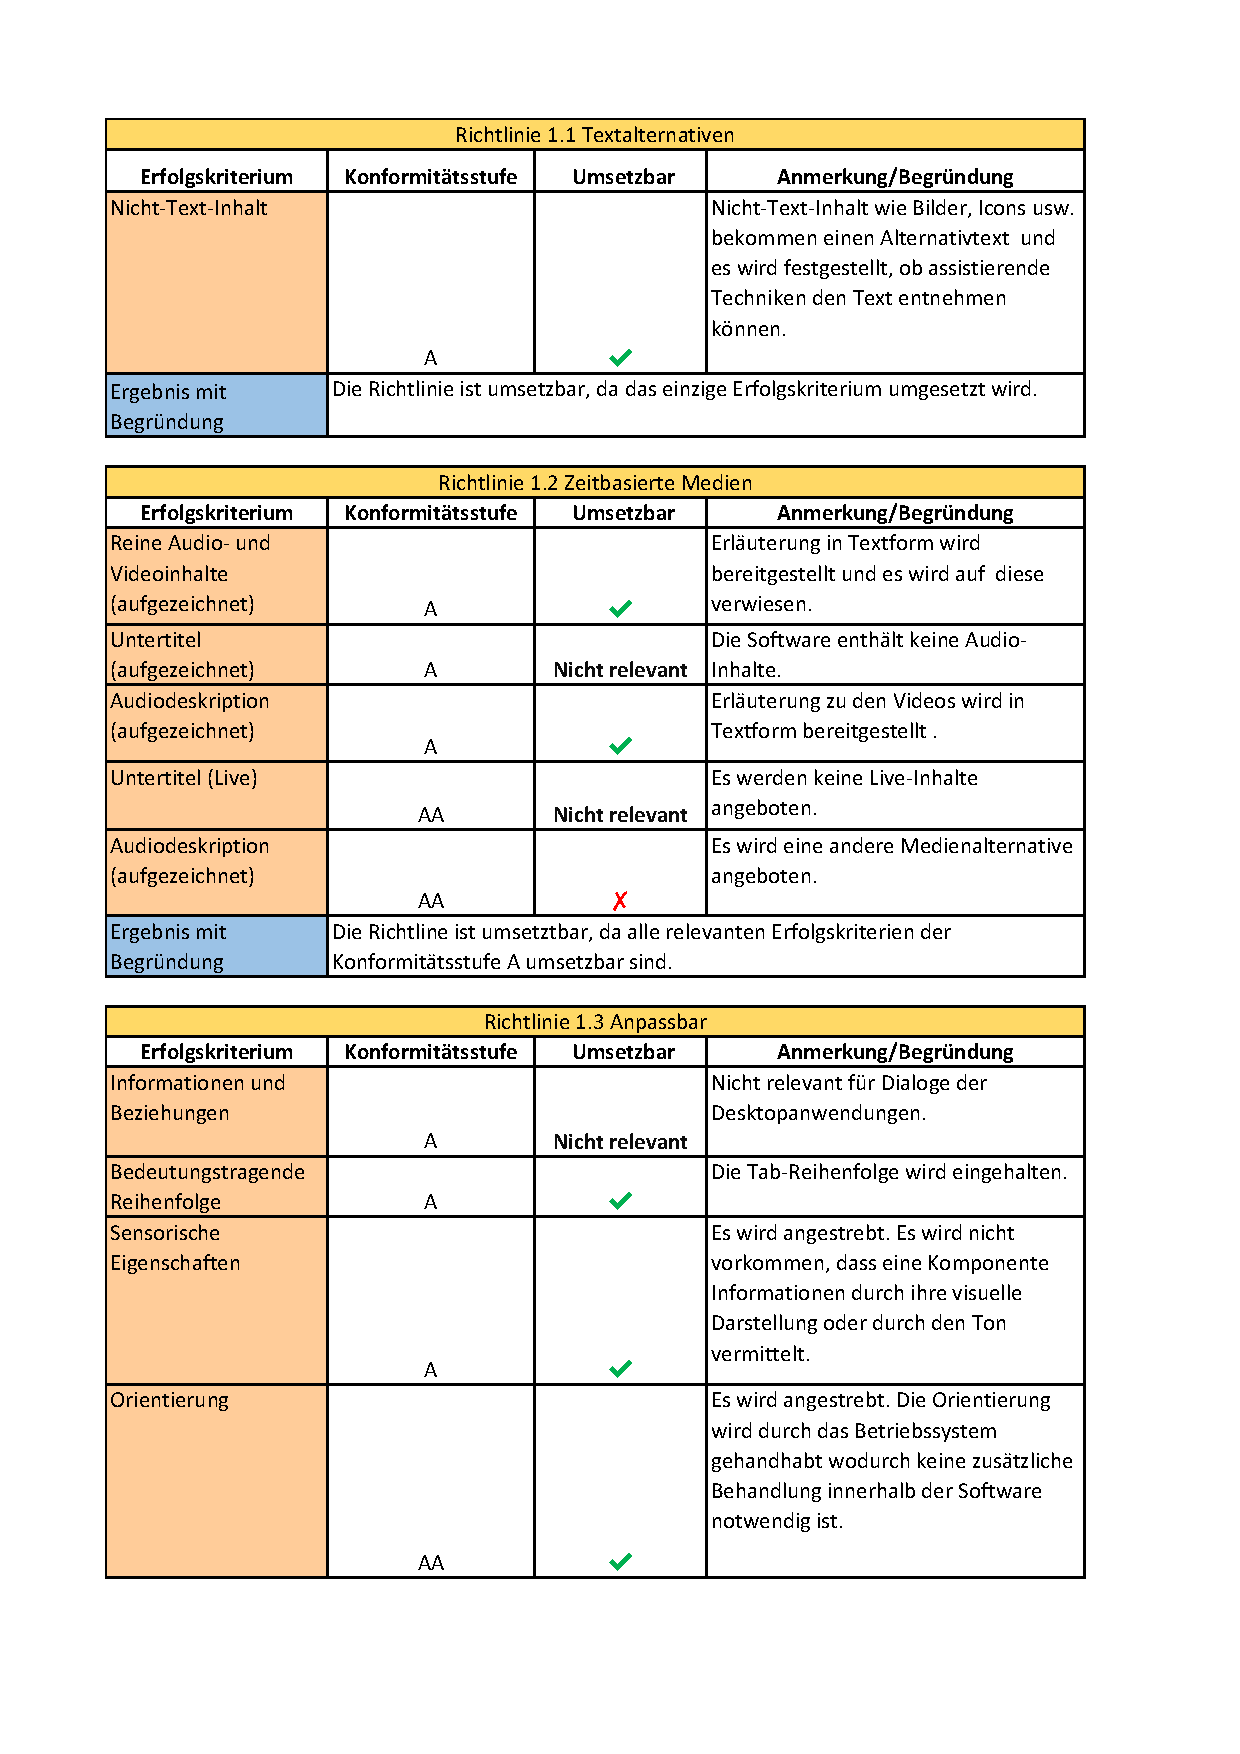
\includepdf[pages=-, scale=0.9, pagecommand={}]{Bewertung der Richtlinien}

\subsubsection{Barrierefreiheit im Software-Entwicklungsprozess}
Beachten die Entwickler die Umsetzung der digitalen Barrierefreiheit von Anfang an nicht, da der Kunde sie im Lastenheft gar nicht verlangt, dann wird eine Umarbeitung der Software sehr aufwendig sein, falls der Kunde sie später doch wünscht.\footnote{Standards für barrierefreie Software \cite{DEVINSIDER}}"`Es empfiehlt sich, bei jeder neuen Entwicklung oder Implementierung, Barrierefreiheit von Anfang an mit zu denken. Zahlreiche Erfahrungen haben gezeigt, dass die Nachrüstung oder Nachbesserung in der Regel deutlich kostenintensiver wird, als die direkte Berücksichtigung."'\footnote{Vgl. Accessibility über Desktopanwendungen hinaus–Barrierefreiheit S. 508 \cite{buhler2017accessibility}}
 
Außerdem ist der Aufwand für das Entwickeln barrierefreier Software von Anfang an geringer als viele Entwickler glauben, da alle  derzeitigen modernen Betriebssysteme globale Funktionen zur Barrierefreiheit anbieten, die der Softwareentwickler dementsprechend nutzen kann, so wie beispielsweise die Bildschirmtastatur, die kontrastreiche Darstellung, die Bildschirmlupe und das Vorlesen von Elementen usw..\footnote{Standards für barrierefreie Software \cite{DEVINSIDER}}

\subsection{Soll-Zustand der Desktopanwendungen}
\label{subsec: Soll-Zustand der Desktopanwendungen}

Aus den Ergebnissen aus dem \cref{subsec: Umsetzbare Kriterien} lässt sich ableiten, dass die Kriterien der \ac{WCAG} 2.0 bzw. der \ac{WCAG} 2.1 für Dialoge der Desktopanwendungen nicht gleich behandelt werden können wie für Webseiten. Es kommt mehr darauf an, welche Aufgaben die Software erledigt, wie viel Dialoge es in der Software gibt und worum es sich im Dialog handelt. Die Umsetzung der Kriterien ist demzufolge vom konkreten Anwendungsfall abhängig und kann nicht auf alle Desktopanwendungen verallgemeinert werden. Schlussendlich hat sich herausgestellt, dass \textbf{14} Kriterien nicht relevant für die Software des Unternehmens sind und \textbf{2} andere Kriterien sind aus bestimmten Gründen nicht umsetzbar, diese wurden dadurch ausgeschlossen. Allerdings gibt es wiederum \textbf{33} Kriterien, die umgesetzt werden können. Die Umsetzung erfolgt jedoch nicht in dieser Arbeit, sondern zu einem späteren Zeitpunkt. Für eine bessere Bearbeitung der umsetzbaren Kriterien wurde ein erster Entwurf eines Katalogs (siehe \nameref{subsec: Anlage5}) erstellt. Dieser Katalog ist Teil der Auswertungstabelle von \cref{subsec: Umsetzbare Kriterien}, allerdings ohne die Kriterien, die in unserem Fall nicht relevant bzw. nicht umsetzbar sind.

Das Ziel der Arbeit ist mit der Erstellung des Katalogs der in Dialogen der Desktopanwendungen umsetzbaren Kriterien erreicht und um das Ganze zu veranschaulichen wurden vier praktische Beispiele aus den aktuellen Dialogen der Software in \nameref{subsec: Anlage4} präsentiert. Diese Beispiele stehen für die Umsetzung folgender Erfolgskriterien:

\begin{itemize}
	\item Text-Kontrast Minimum
	\item Tastatur-Kurzbefehle
	\item Fehlererkennung
	\item Linkzweck
\end{itemize}

Jeder Dialog der aktuellen Desktopanwendungen wird in Zukunft auf die Erfüllung der umsetzbaren Kriterien getestet. Es wurde im Rahmen dieser Arbeit nicht getestet, ob alle Dialoge momentan die erwähnten Beispiele (siehe \nameref{subsec: Anlage4}) erfüllen.